\documentclass[Rapport/Rapport_main.tex]{subfiles}
\begin{document}
\subsection{BallDispenser Controller}
\subsubsection{Softwaredesign}
Denne komponenten er hoved kontrollen til ballDispenser, den er ansvarlig for styre både coinDispenser og ballDispenser. Den indeholder også funktionene som kreves får å sende og motta beskjeder til RPi. Dens hoved funksjon er coinInserted den kan sees under (Listing \ref{lst:dispenserControlFunction}). 
\begin{lstlisting}[caption={Hoved kontrol funksjonen til ballDispenser},style=customc,label={lst:dispenserControlFunction}]
void coinInserted()
{
    handleCoinDetection();
    if(countBalls() <= 2)
        {
            disableDispenser(); 
            sendDispenserStatus();
        }
    sendCoinDetected();
    dispenseBalls();
    resetDetectionISR();
}
\end{lstlisting}

For å opprette kommunikasjonen mellom BallDispenser og RPi brukes I2C slave modulet som er et modul fra PSoC Creator og et interrupt som trekkes lavt når BallDispenser har en melding som skal sendes til RPi.
\begin{figure}[H]
    \centering
    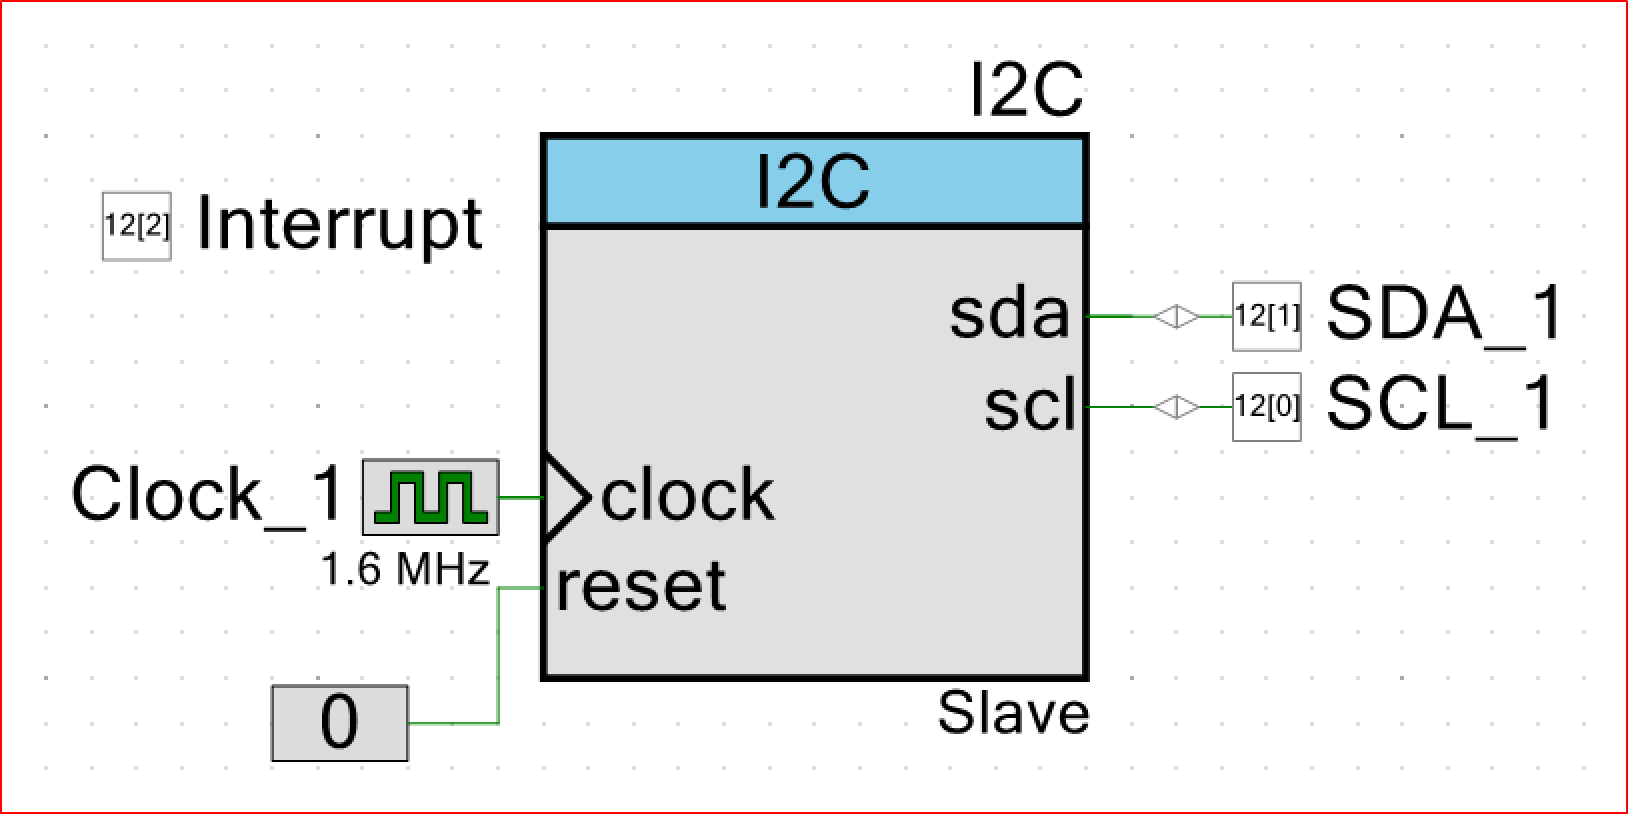
\includegraphics[width=\textwidth]{Rapport/BallDispenser/ballDispenserController/graphics/I2Cslave.png}
    \caption{I2C slave modul}
    \label{fig:I2CSlaveBallDisp}
\end{figure}

\subsubsection{Implementering}
Implementeringen av CoinDispenser er skrevet i C med bruk av PSoC Creator som er utviklings plattformen til PSoC.
\end{document}